\beginsong{Ein Krampenschlag vor Tag}[wuw={Theodor Kramer, Thomas Fritz, 1934}, bo={356}, index={Was bin ich nur so jäh erwacht}]

\markboth{\songtitle}{\songtitle}

\beginverse
\endverse

\centering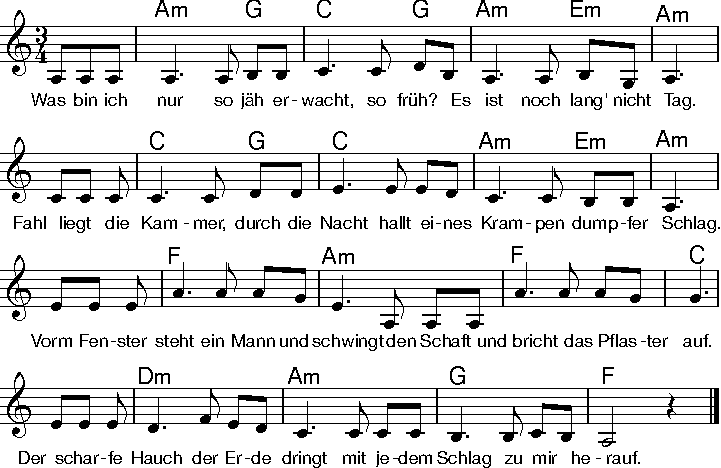
\includegraphics[width=1\textwidth]{Noten/Lied033.pdf}	

\beginverse
Vor Schwäche \[Am]dreht es \[G]mich zur \[C]Wand; lang \[G]ist es \[Am]her, schon \[Em]viel zu \[Am]lang,
dass auf dem \[C]Steig ge\[G]spreizt ich \[C]stand bei Nacht und \[Am]selbst den \[Em]Krampen \[Am]schwang.
Die Funken \[F]stoben und wie \[Am]Wein roch scharf der \[F]Grund, das ist vor\[C]bei.
Ein and'rer \[Dm]lockert Stein um \[Am]Stein und weckt mich \[G]vor dem Hahnen\[F]schrei.
\endverse 

\beginverse
Der du vor'm ^Fenster ^stehst, viel^leicht hab' ^ich vor ^Jahren ^dich ge^kannt
und dir die ^Schaufel ^zuge^reicht und hab' dich ^meinen ^Freund ge^nannt.
Das ist vor^bei, lang hungert ^mich. Ich tät' dein ^Werk genauso ^gut.
Und säh' ich ^auf der Straße ^dich, ich zöge ^nicht vor dir den ^Hut.
\endverse

\beginverse
Weißt du, Ge^sell, was ^Hunger ^ist? Und ^weißt du's ^auch, was ^gilt es ^mir!
Den Karren, ^der die ^Erde ^frisst, das Scheit, den ^Krampen ^neid' ich ^dir.
Ich ließ dich ^nicht herein zur ^Tür; du reißt mit ^jedem neuen ^Schlag,
kannst du auch ^zehnmal nichts da^für, mehr als das ^Pflaster auf vor ^Tag.
\endverse

\beginverse
Den tiefen ^Riss, du ^schüttest ^nicht, so^lang du ^lebst, mit ^nichts ihn ^zu.
Am Barren ^schwingt das ^rote ^Licht, die fahlen ^Sterne ^geh'n zur ^Ruh'.
Ein Zug geht ^draußen auf dem ^Steig verhallt der ^letzte Krampen^schlag;
ans Fenster ^schlägt ein schwarzer ^Zweig, mich friert, es ^ist noch lang nicht \[Am]Tag.
\endverse

\endsong

\beginscripture{}
Krampen = Spitzhacke; Das Lied behandelt die Problematik der Arbeitslosigkeit, indem es dem fortwährend Arbeitenden mit der Krampe einen unbeschäftigten, schlaflosen Zuhörer entgegensetzt.
\endscripture

\begin{intersong}

\end{intersong}